

\section{Experimental Setup}
\label{sec:experimental-setup}\label{sec:exp-setup}

\begin{figure}[htbp]
  \centering
  \vspace{-0.1in}
  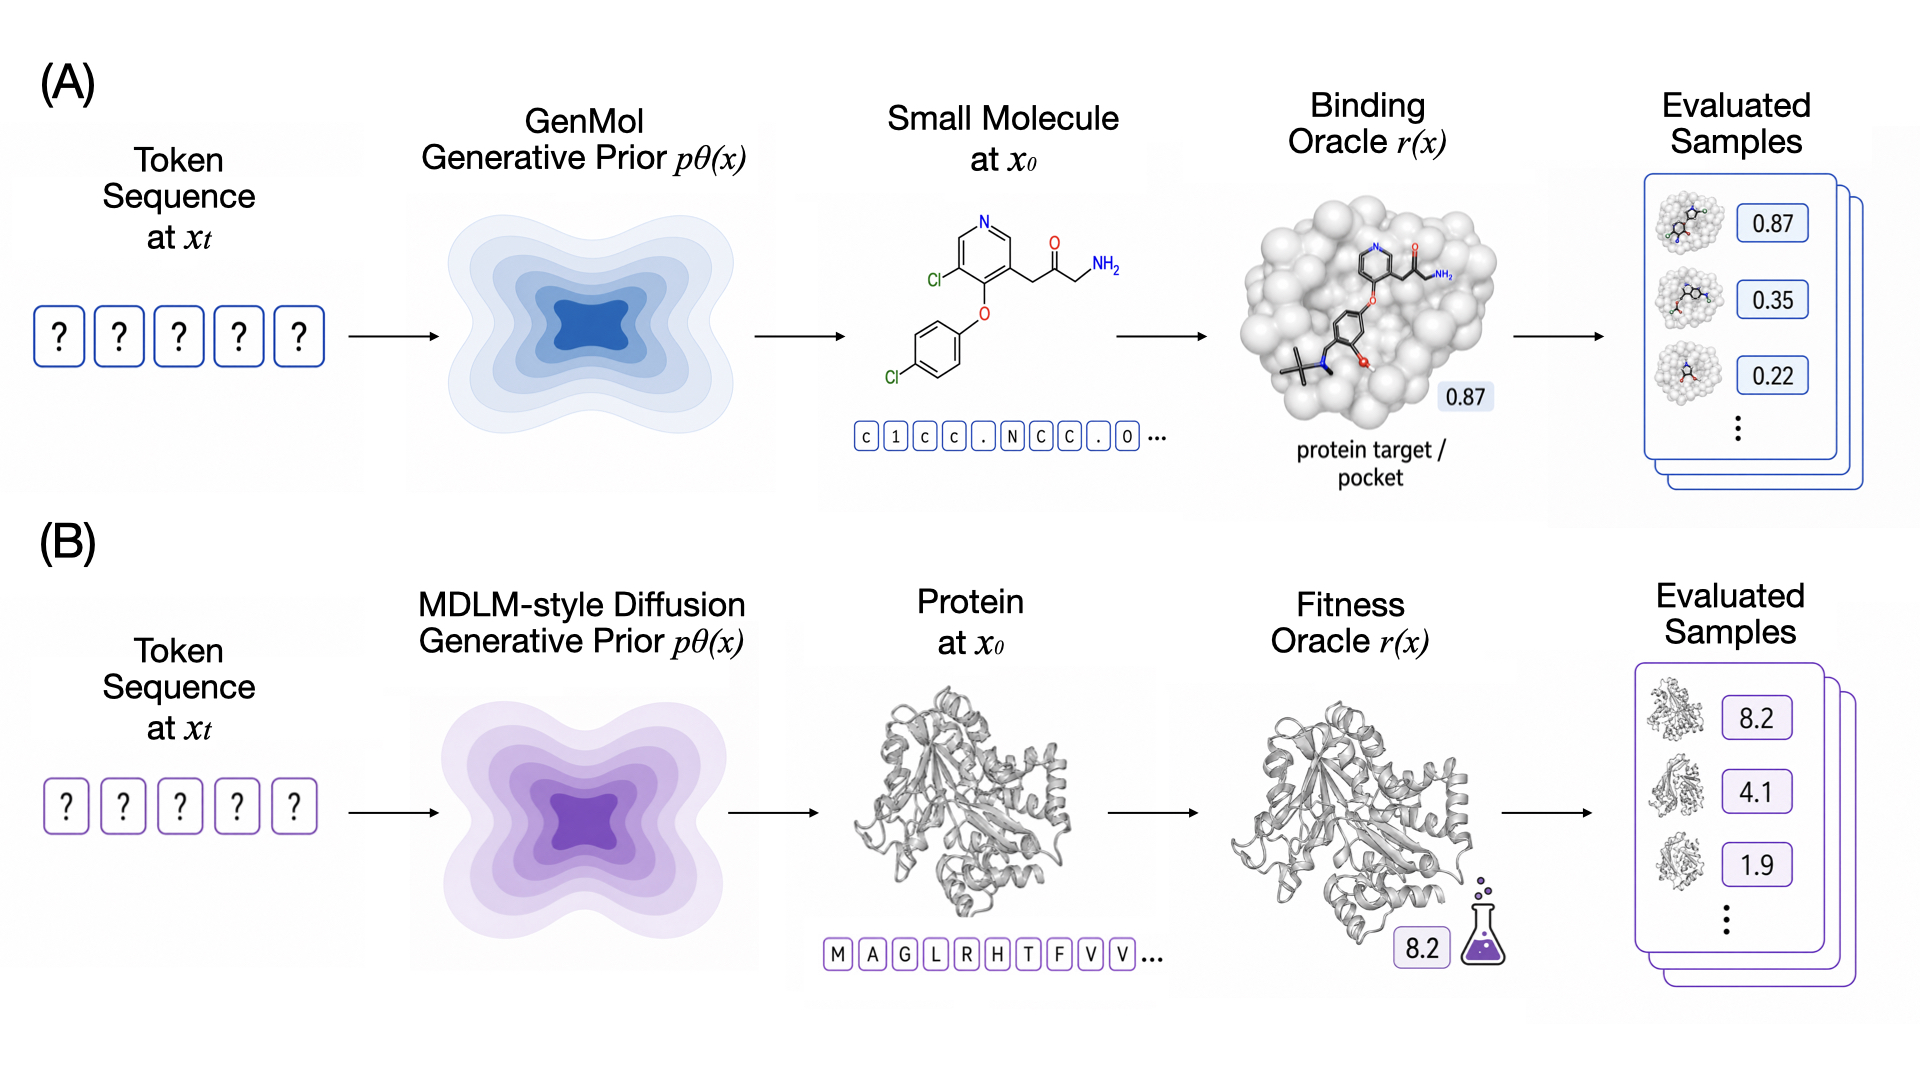
\includegraphics[width=\textwidth]{figures_source/Applications002.jpeg}
  \vspace{-0.4in}
  \caption{In this study, we explore several tasks across two different domains, optimizing \textbf{(A)} small molecules for binding to protein targets and \textbf{(B)} proteins for various fitness metrics.}
  \vspace{-0.1in}
  \label{fig:diag_domain}
\end{figure}

\textbf{Tasks and oracles.}
We evaluate whether the design choices in Section~\ref{sec:design-space} improve discovery utility of finetuning methods under a fixed test-time budget. We study nine molecular optimization tasks across two domains. (Fig.~\ref{fig:diag_domain}) The first domain is small-molecule optimization for binding affinity to six protein targets (2VT4, 5SDV, 6CM4, 7BKC, 7C7M, 7YLL from \citep{zhangODesignWorldModel2025}) with GenMol \citep{leeGenMolDrugDiscovery2025} as the generator and FlashAffinity (FA) \citep{jiangFlashAffinityBridgingAccuracySpeed} as the primary oracle, with selected comparisons re-run under Boltz-2 \citep{passaro2025boltz2} to verify conclusions hold for an oracle two orders of magnitude more expensive and more accurate. While many studies approach this from a structure-based generative design perspective \citep{zhangODesignWorldModel2025, zengPropMolFlowPropertyguidedMolecule2026, schneuingStructurebasedDrugDesign2022,  guan3DEquivariantDiffusion2023, rekeshSynCoGenSynthesizable3D2025, adamsShEPhERDDiffusingShape2025}, we use discrete diffusion due to the increased validity, synthesizability, and diversity of generations offered by these models. The second domain is protein fitness optimization across three families (GB1, CreiLOV, TrpB) with a per-family MDLM-style discrete diffusion generator \citep{sahooSimpleEffectiveMasked2024} and a per-family fitness surrogate trained from experimental measurements as the oracle \citep{yangSteeringGenerativeModels2025}. For finetuning, we use either DDPP \citep{rector-brooksSteeringMaskedDiscrete2024} or VIDD \citep{suIterativeDistillationRewardGuided2025}. The complete environment is detailed in Appendix~\ref{app:repro-recipe}.


\textbf{Rewards.} In both domains the oracle \emph{defines} the reward the algorithm optimizes, and we treat it as ground truth in place of an expensive assay. For a molecule $x$ and target $p$, the reward is the molecular-weight-corrected, negated FA value head, $r(x) = -\mathrm{MWcorr}\bigl(\mathrm{FA}_{\text{val}}(x, p)\bigr)$, so that larger means stronger predicted binding; it is an unbounded affinity value rather than a normalized score, which is why absolute rewards differ across targets and we only ever compare within a target. For proteins the reward is the per-family fitness predictor: predicted IgG-Fc binding/enrichment fitness for GB1, predicted fluorescence fitness for CreiLOV, and predicted catalytic fitness for tryptophan formation from indole and serine for TrpB. Higher is better in all cases.


\textbf{Experimental protocol.} The high-level stages in Fig.~\ref{fig:test_time_feedback} define our \emph{full method} configuration for online adaptation, which serves as the upper-bound reference point for every ablation in Sec.~\ref{sec:results}. Each round generates $M$ candidates from the current $p_{\theta_t}$, selects the top-$K$ candidates ranked by Thompson-sampled surrogate scores for oracle evaluation, applies the invalid-SMILES penalty to candidates that fail RDKit before they reach the oracle, refreshes the CVaR threshold $\tau$ from the buffer, and runs $G$ fine-tuning gradient steps on stratified mini-batches with both reward-shape knobs (CVaR $+$ Density Entropy Regularization) applied to the log-reward. The ensemble surrogate is refit on the accumulated pairs at the end of each round. Pseudocode for the loop is given in Appendix~\ref{app:diagrams} as Algorithm~\ref{alg:method}.

\textbf{Evaluation protocol.}
Each method is evaluated under the same oracle-evaluation budget $B$ and random seeds. We report performance both as a function of cumulative oracle calls and as a function of GPU hours. Our primary metrics measure the upper tail of the evaluated set $\mathcal{D}_B$. We primarily report the best reward discovered so far, $\max_{x\in\mathcal{D}_B} r(x)$, as well as top-$k$ and top-$k\%$ means. To compare across tasks, we report the \emph{normalised reward}
\begin{equation}
\mathrm{NR}_t(x) \;=\; \frac{r_t(x)-C_t}{F_t-C_t},
\label{eq:lift}
\end{equation}
where $r_t(x)$ is the raw score of method $x$ on target $t$ at the evaluated budget, and $C_t$ and $F_t$ are target-specific reference endpoints computed over the methods in the corresponding comparison. Because raw FA rewards are unbounded and vary in scale across targets, this within-paper normalisation maps each target's reference interval to $[0,1]$, allowing aggregation across heterogeneous tasks. Since it is relative to the evaluated method set, it is intended for within-paper aggregation rather than cross-paper comparison. Alongside normalised reward, which evaluates vertical slices of the trajectory at a fixed budget $B$ to measure discovery quality, we report oracle-call speedup, which evaluates horizontal slices at a fixed target score (specifically, the strongest baseline's terminal score) to measure feedback efficiency. Because reward optimization can exploit oracle artifacts or leave the valid molecular manifold, we additionally track secondary metrics over a sliding window of generated candidates (parameters in Appendix~\ref{app:traces}): SMILES validity, pairwise Tanimoto diversity \citep{bajusz2015tanimoto}, QED \citep{bickerton2012qed}, and SA \citep{ertl2009sa}. We compare the full online loop against unconditional sampling, inference-time search variants, offline fine-tuning, and online fine-tuning without plug-in components (the untreated/vanilla
DDPP-LB or VIDD baseline).

\textbf{Advanced search.}
In addition to the core acquisition choice above, we also test whether the candidate-generation step benefits from inference-time search. Instead of plain ancestral sampling from the current generator, the loop can propose candidates using beam search \citep{ramesh2025noisetrajectory}, MCTS \citep{tangTR2D2TreeSearch2025}, or discrete Feynman-Kac correction \citep{hasanDiscreteFeynmanKacCorrectors2026, skretaFeynmanKacCorrectorsDiffusion2025} guided by the reward surrogate \citep{yangSteeringGenerativeModels2025}. In recent years, there have been significant related efforts combining inference time guidance with a fixed generator, which we do not fully explore here \citep{didi2026scaling, wangFineTuningDiscreteDiffusion2024, singhalGeneralFrameworkInferencetime2025, liDerivativeFreeGuidanceContinuous2024, nisonoffUnlockingGuidanceDiscrete2025, gruverProteinDesignGuided2023,  xiongProteinGuideOntheflyProperty2026, luProVADAGenerationSubcellular2025, ueharaRewardGuidedIterativeRefinement2025, liDynamicSearchInferenceTime2025, jianGeneralBindingAffinity2026, yangHitLeadDiscovery, tangPepTuneNovoGeneration2024, tangTR2D2TreeSearch2025, yangSteeringGenerativeModels2025}.
